In a diffraction tube, electrons accelerated through a voltage $U$ pass a thin graphite foil. On the screen, $L = \LsO$ behind the foil, they make rings. The radius $r$ of the inner ring is measured for several voltages:

\begin{center}
\begin{tabular}{l|ccccc}
$U$ in \si{\kilo\volt} & 2.5 & 3.5 & 4.0 & 4.5 & 5.0 \\ \hline
$r$ in \si{\milli\meter} & 15.8 & 13.1 & 12.1 & 11.6 & 11.0
\end{tabular}
\end{center}

In the graph, $r$ is plotted against $1/\sqrt{U}$.

\begin{center}
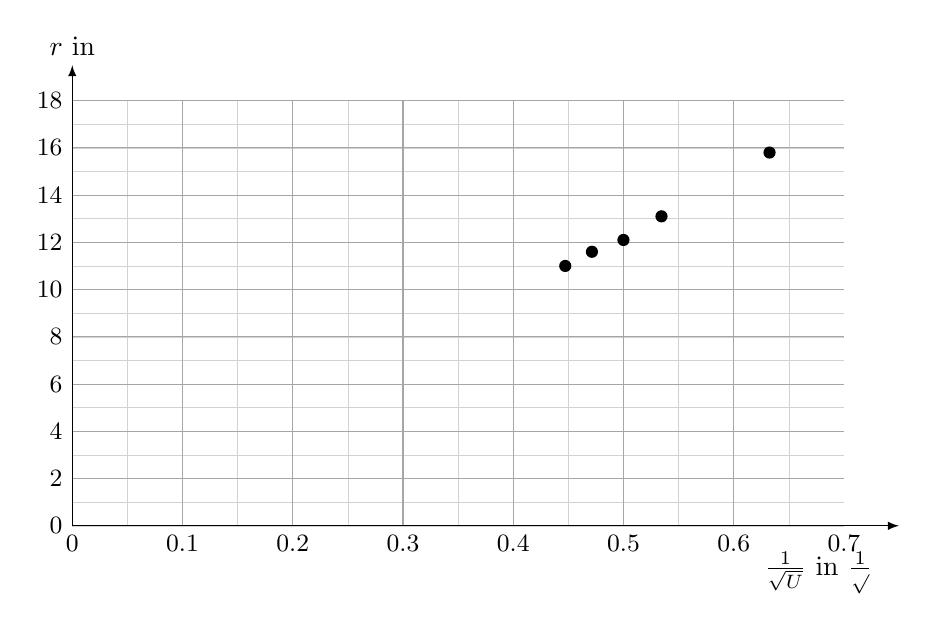
\begin{tikzpicture}[x=14cm, y=0.3cm, >=latex]
 \draw[gray!35, very thin] (0,0) grid[xstep=0.05, ystep=1] (0.7,18);
 \draw[gray!70] (0,0) grid[xstep=0.1, ystep=2] (0.7,18);
 \draw[->] (0,0) -- (0.75,0) node[below left=6pt] {$\frac{1}{\sqrt{U}}$ in $\frac{1}{\sqrt{\si{\kilo\volt}}}$};
 \draw[->] (0,0) -- (0,19.5) node[above] {$r$ in \si{\milli\meter}};
 \foreach \x in {0,0.1,0.2,0.3,0.4,0.5,0.6,0.7} \node[below] at (\x,0) {\small \x};
 \foreach \y in {0,2,...,18} \node[left] at (0,\y) {\small \y};
 \fill (0.6325,15.8) circle (2.2pt);
 \fill (0.5345,13.1) circle (2.2pt);
 \fill (0.5000,12.1) circle (2.2pt);
 \fill (0.4714,11.6) circle (2.2pt);
 \fill (0.4472,11.0) circle (2.2pt);
\end{tikzpicture}
\end{center}

\begin{abcliste}
\abc Calculate the wavelength of the electrons at \UAO.
\abc The ring comes from lattice planes of the graphite at the spacing $d$. The beam is deflected by twice the Bragg angle, so for small angles $r/L = \lambda/d$. Show that the points should lie on a line through the origin, and find $d$ from its slope.
\abc The voltage is made four times as large. How does the radius of the ring change?
\end{abcliste}
